\subsection{Decision ontology pattern} \label{odp_decision_ontology}
% Subsection structure:
% Problem: what is the generalized problem?
% 	Motivation: why is this problem scientifically important and/or interesting?
% Solution: conceptual description of solution, including formal definition of GODP and SHACL shapes.
% 	Illustration: images of GODP structure.
% 	(Statistical)Analysis: how does the solution solve the problem?
% 	Evaluation: are the results significant? What is the impact?
\subsubsection{An information maturity-level structure}
The evidence-based management, completeness, reproducibility, consensus, and conflict patterns solve separate generic problems. At the same time, these patterns overlap in their ontology structure. This overlap makes it difficult to use these patterns in the same environment. The decision design pattern provides the glue between the completeness, reproducibility, consensus, and conflict patterns, using the evidence-based management pattern as a base. 

The decision presentation pattern combines the output from the completeness, reproducibility, consensus, and conflict patterns to calculate the \emph{information maturity-level} for a decision. The decision-maker needs to make a \emph{meta-decision} based on the information maturity-level:
\begin{enumerate}
\item If the information maturity-level is acceptable, the decision-maker can make the main-decision.
\item If the information maturity-level is not acceptable, the decision-maker needs to increase the information maturity-level until it is acceptable.
\end{enumerate}

The outcome of the meta-decision depends on the complexity and impact of the main-decision. If the complexity and impact of the main-decision are low, a lower information maturity-level might be acceptable. However, if the impact and complexity of the main-decision are high, we expect that the requirements towards the information maturity-level are higher as well. 

\begin{center}
\large\color{document}{The decision ontology pattern increases the transparency of the completeness and reliability of decision-relevant information.} 
\end{center}

The scale of the impact and complexity of a decision are organisation dependent. For example, a C-level decision in an organisation with 3000 employees has a different impact compared to a C-level decision in an organisation with 300 employees. As a result, we cannot automate this meta-decision. In essence, a human needs to evaluate, based on knowledge and experience, if the complexity and impact of the decision justify the information maturity-level.

\subsubsection{Completeness} \label{odp_completeness}
% Subsection structure:
% Problem: what is the generalized problem?
% 	Motivation: why is this problem scientifically important and/or interesting?
% Solution: conceptual description of solution, including formal definition of GODP and SHACL shapes.
% 	Illustration: images of GODP structure.
% 	(Statistical)Analysis: how does the solution solve the problem?
% 	Evaluation: are the results significant? What is the impact?
\paragraph{Detecting completeness}
A decision-maker makes a decision knowing context-relevant information for that specific decision. Some information crucial for decision $x$ might be irrelevant for decision $y$. Each decision requires different context-relevant information. This pattern allows a domain expert to define the context-relevant information.

\begin{center}
\large\color{document}{The completeness pattern validates the completeness of information by detecting missing information.}
\end{center}

\paragraph{Ontology}
The completeness pattern detects if an individual classified as $C$ is incomplete, considering a required property $p$. We achieve this by creating a data property or an object property and use parameters to define its domain and range. The constraints detect individuals classified as $C$ that do not host the data or object property. The detected individuals are considered incomplete and, therefore, premature.

\paragraph{Inferencing}
The completeness pattern infers the class of individuals from the domain or range of the data or object property. For example, if $Information$ is the domain of the property $data\_description$, then the reasoner will infer individuals that have a $data\_description$ as $Information$. Figure \ref{fig:04_data_description} presents this example in Prot\'eg\'e.

\begin{figure}[H]
\centering
  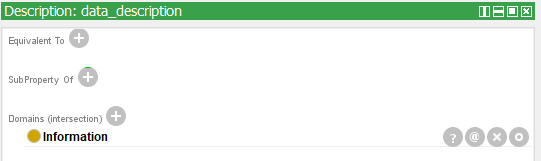
\includegraphics[width=10cm]{../../Images/04_Contribution/04_data_description.png}
  \caption{If $Information$ is the domain of the property $data\_description$, then the reasoner will infer individuals that have a $data\_description$ as $Information$.}
  \label{fig:04_data_description}
\end{figure}

\paragraph{Inconsistency}
Code sample \ref{GODP_COMP} presents the generic ontology design pattern to create a data property. This code sample includes a range. The definition of the range limits the data range that the data property accepts, for example, a $xsd:string$ accepts strings or $xsd:int$ accepts integers. The ontology is inconsistent when the data property stores a value that is outside of the defined range.

\paragraph{Generic ontology design pattern}
Code sample \ref{GODP_COMP} adds a data property or an object property to an existing class. We use three parameters to instantiate the data or object property: $c$ defines the class that should host the data property, $p$ defines the data property itself, and $r$ defines the range of the data property. We use the range of the data property to restrict its content using, for example, regular expressions and use the range of the object property to infer the class of an individual. Figure \ref{fig:GODP_COMP_DP} presents the data property, and figure \ref{fig:GODP_COM_OP} presents the object property.

\begin{lstlisting}[float,language=GDOL,caption={The GDOL code for adding a required data property to an existing class using two parameters. We use $c$, $i$, and $r$ as parameters to instantiate the data or object property.},label={GODP_COMP}][H]
pattern Completeness_dp [Class: c; DataProperty: i; Datatype: r] =
	DataProperty: i Domain: c Range: r
pattern Completeness_op [Class: c; ObjectProperty: i; Datatype: r] =
	ObjectProperty: i Domain: c Range: r
\end{lstlisting}

\begin{figure}[H]
\centering
  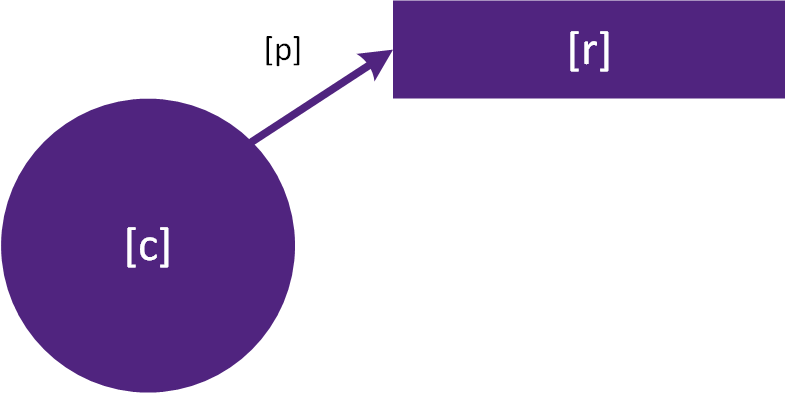
\includegraphics[width=5cm]{../../Images/04_Contribution/Completeness_DP.png}
  \caption{The completeness of a class using a data property. Code sample \ref{GODP_COMP} presents the GDOL code for adding a data property to an existing class. Code sample \ref{GODP_COMP} presents the GDOL code that instantiates this ontology.}
  \label{fig:GODP_COMP_DP}
\end{figure} 

\begin{figure}[H]
\centering
  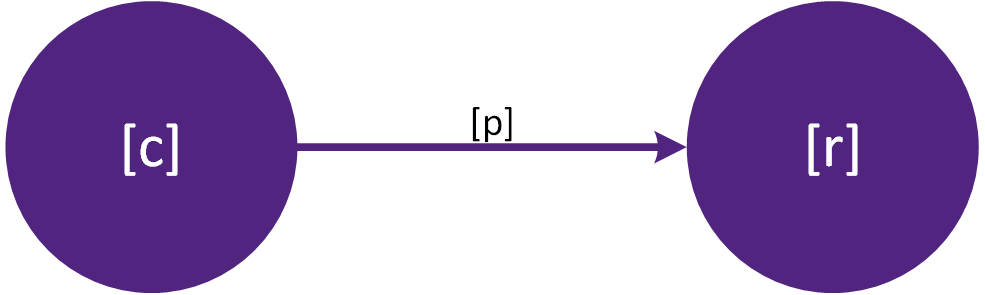
\includegraphics[width=6cm]{../../Images/04_Contribution/Completeness_OP.png}
  \caption{The completeness of a class using an object property. Code sample \ref{GODP_COMP} presents the GDOL code for adding an object property to an existing class. Code sample \ref{GODP_COMP} presents the GDOL code that instantiates this ontology.}
  \label{fig:GODP_COM_OP}
\end{figure} 

\paragraph{Constraints}
The SHACL shape in code sample \ref{SHACL_COM_DP} detects when an individual classified as $c$ does not host the defined data or object property $p$. Each individual classified as $c$ should have at least one path (object or data property) $p$. The SHACL shape monitors the existence of the data or object property using the cardinality constraint $minCount$. $c$ and $p$ set the context of the constraints.

\begin{lstlisting}[float,language=SHACL,caption={The SHACL code that validates if the individuals classified as $c$ host the property $p$. We use the cardinality constraint $sh:minCount$ for this detection: each individual classified as $c$ should have at least one path (object or data property) $p$.},label={SHACL_COM_DP}][H]
[c]Shape a sh:NodeShape;
	sh:targetClass [c]; 
	sh:property [
		sh:path [p]; 
		sh:severity sh:Violation; 
		sh:minCount 1; 
		sh:message "Completeness: add [c] to [p]."; ]
\end{lstlisting} 
\subsubsection{Reproducibility} \label{odp_reproducibility}
% Subsection structure:
% Problem: what is the generalized problem?
% 	Motivation: why is this problem scientifically important and/or interesting?
% Solution: conceptual description of solution, including formal definition of GODP and SHACL shapes.
% 	Illustration: images of GODP structure.
% 	(Statistical)Analysis: how does the solution solve the problem?
% 	Evaluation: are the results significant? What is the impact?
\paragraph{Detecting reproducibility}
We use reproducibility to evaluate the reliability of decision-relevant information. The reproducibility pattern can detect when information cannot be traced back to an evidence source. When evidence cannot be traced back to an evidence source, the pattern detects the information as premature. 

\begin{center}
\large\color{document}{The reproducibility pattern validates the information reliability by detecting when information cannot be traced back to an evidence source.}
\end{center}

\paragraph{Ontology}
Information is reproducible when it can be traced back to evidence or an information source, for example, a contextual circumstance or the value of a stakeholder. This pattern relates information to an evidence source using an object property. An information class can be based on another information class as well, as long as the chain of information is evidence-based. We use the completeness pattern to ensure the required data properties are available. Figure \ref{fig:reproducibility_chain} presents a chain that connects information to evidence. The $based\_on\_in{\f}ormation$ object property is transitive. When we base information $a$ on information $b$, and information $b$ on information $c$, then information $a$ is also based on information $c$. We need the transitive characteristic to query the evidence sources of information for the decision presentation pattern.

\begin{figure}[H]
\centering
  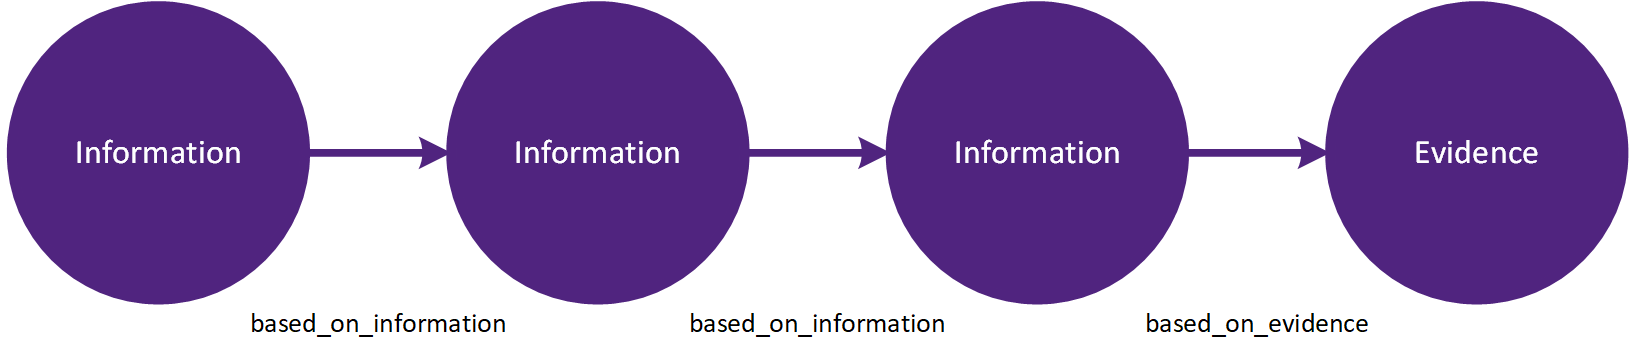
\includegraphics[width=13cm]{../../Images/Reproducibility_Chain.png}
  \caption{An example of an evidence-based chain of information. The reproducibility pattern should detect if the information in the chain is not evidence-based.}
  \label{fig:reproducibility_chain}
\end{figure} 

We extend the evidence-based management pattern in two ways:
\begin{enumerate}
\item Contextual circumstances and evaluated external evidence naturally refer to their actual evidence source, for example, a scientific article or an observation. Stakeholder evidence requires a specific stakeholder as a source of evidence. We extend the evidence-based management pattern with one class ($Stakeholder$) and the related object property ($shared\_by$). 
\item Individuals (classified as $In{\f}ormation$) hosting data properties should be evidence-based or information-based. The object property $based\_on\_evidence$ relates a class to the evidence class. The object property $based\_on\_in{\f}ormation$ relates a class to an information class. 
\end{enumerate} 

Figure \ref{fig:reproducibility} presents the resulting ontology. We have marked the extensions of the evidence-based management pattern in \textcolor{DarkBlue}{blue}.

\begin{figure}[H]
\centering
  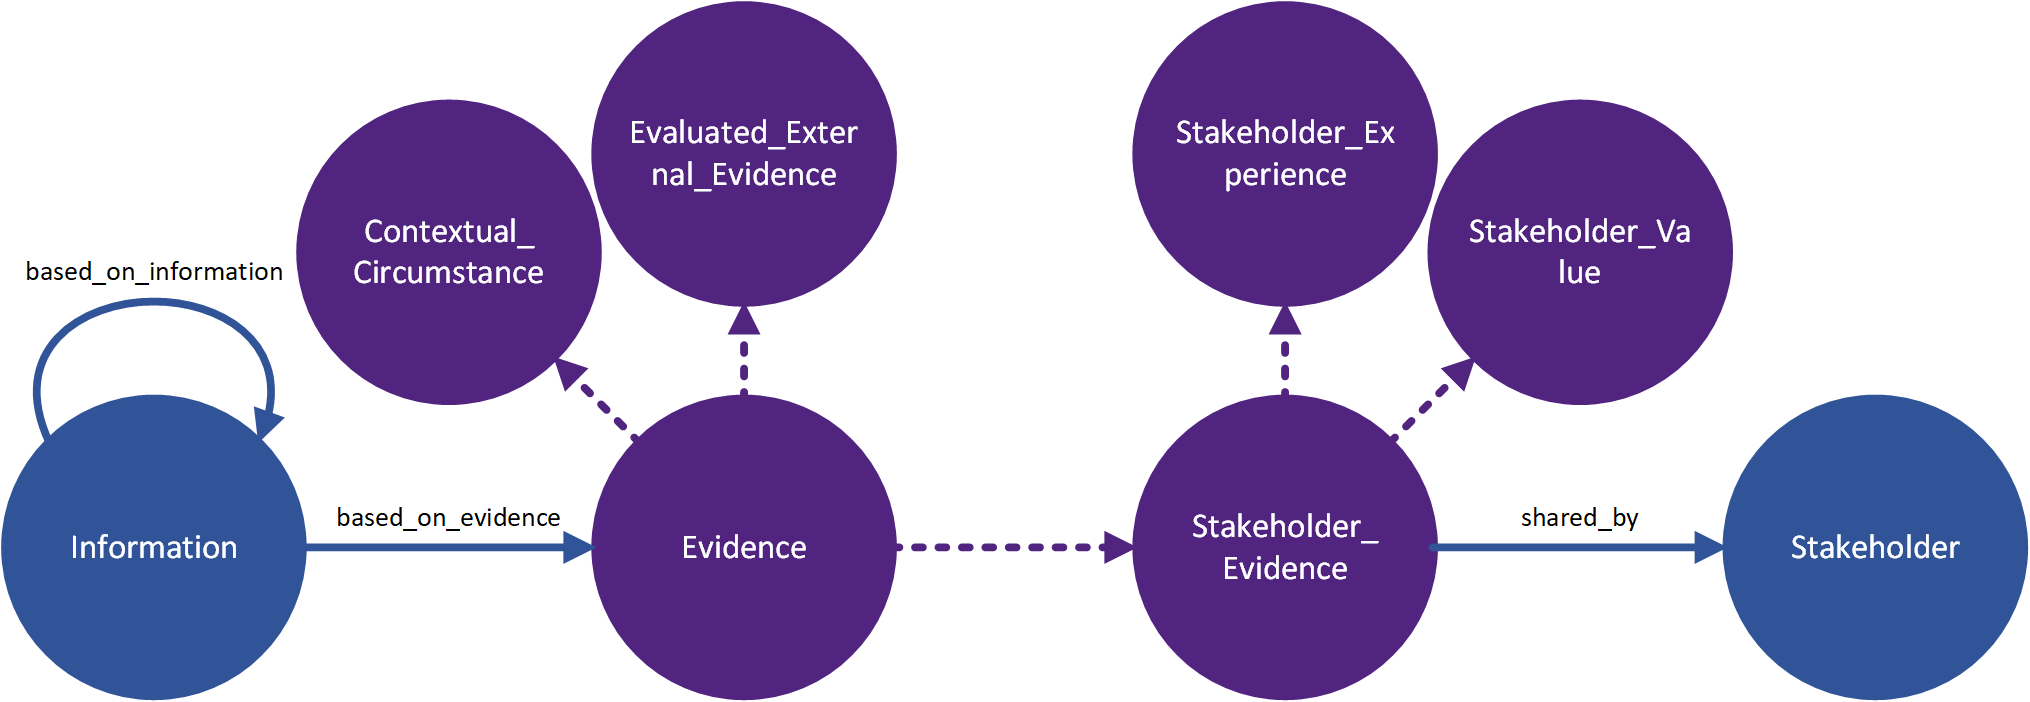
\includegraphics[width=14cm]{../../Images/04_Contribution/04_Reproducibility_Ontology.png}
  \caption{The reproducibility ontology. We have marked the extensions of the evidence-based management pattern in \textcolor{DarkBlue}{blue}. Code sample \ref{GODP_REP_EXT} presents the GDOL code that we use to instantiate this pattern.}
  \label{fig:reproducibility}
\end{figure}

\paragraph{Inferencing}
We use the domain and range of the $based\_on\_information$, $based\_on\_evidence$, and $shared\_by$ object properties to allow the reasoner to classify individuals that are using these object properties. Table \ref{table:rep_inference} presents the classification the reasoner infers from the domain and range configuration.

\begin{table}[H]
\centering
\caption{We use the domain and range of the $based\_on\_in{\f}ormation$, $based\_on\_evidence$, and $shared\_by$ object properties to allow the reasoner to classify individuals that are using these object properties.}
\begin{tabular}{| p{4cm} | p{6cm} |  p{4cm} |   }
\hline
\rowcolor{document}
\color{documentText}Domain & \color{documentText}Object property & \color{documentText}Range \\
\hline
$In{\f}ormation$ & $based\_on\_in{\f}ormation$ & $In{\f}ormation$ \\
\hdashline
$In{\f}ormation$ & $based\_on\_evidence$ & $Evidence$ \\
\hdashline
$Stakeholder\_Evidence$ & $shared\_by$ & $Stakeholder$ \\
\hline
\end{tabular}
\label{table:rep_inference}
\end{table}

\paragraph{Inconsistency} \label{rep_incons}
We guard the consistency of the ontology using $DisjointClasses$. The reasoner cannot classify an individual as $Information$ and $Evidence$ at the same time. If we allow the reasoner to do this, it might create a circular dependency in the reproducibility chain figure \ref{fig:reproducibility_chain} presents. $In{\f}ormation$ typically represents a statement that we can trace back to at least one $Evidence$ source. Code sample \ref{GODP_REP_EXT} presents the implementation of the $DisjointClasses$.

\paragraph{Generic ontology design pattern}
Figure \ref{fig:reproducibility} presents an ontology that extends the evidence-based management ontology and enables the detection of unreproducible information. Code sample \ref{GODP_REP_EXT} presents the GDOL code that extends the evidence-based management ontology. 

\begin{lstlisting}[float,language=GDOL,caption={The GDOL code for relating information to evidence and stakeholder evidence to a stakeholder. We introduce two new classes ($Stakeholder$ and $Information$) and three new object properties ($shared\_by$, $based\_on\_evidence$, and $based\_on\_in{\f}ormation$. Additionally, we define that $Information$ and $Evidence$ are disjoint. Figure \ref{fig:reproducibility} visualises the result of executing the code.},label={GODP_REP_EXT}][H]
ontology Reproducibility_Basic = EBM then 
 Class: Stakeholder 
 Class: Information 
 ObjectProperty shared_by Domain: Stakeholder_Evidence Range: Stakeholder 
 ObjectProperty based_on_evidence Domain: Information Range: Evidence
 ObjectProperty based_on_information Domain: Information Range: Information Characteristics: Transitive
 DisjointClasses: Information, Evidence
\end{lstlisting}

The classes that store decision-relevant information are required to be a subclass of $In{\f}ormation$. Code sample \ref{GODP_REP_EV} presents the GDOL code that relates information to evidence. The inferencing using the domain and range of the $based\_on\_in{\f}ormation$, $based\_on\_evidence$, and $shared\_by$ object properties contributes to this classification as well.

\begin{lstlisting}[float,language=GDOL,caption={The GDOL code that classifies individuals as a sub-class of $Information$. We use $dri$ (decision relevant information) and $i$ (information) as parameters.},label={GODP_REP_EV}][H]
pattern Reproducibility_Context [Class: dri; Class: i] = 
 Class: [dri] SubClassOf: [i]
\end{lstlisting}

\paragraph{Constraints}
Code sample \ref{SHACL_REP} presents the SHACL shape that detects unreproducible information. Each individual that is classified as $In{\f}ormation$ is required to host the object property $based\_on\_in{\f}ormation$ or $based\_on\_evidence$. Individuals that are classified as $In{\f}ormation$ can be traced back to an evidence or information source by hosting one of these two object properties. If the individual does not host one of the object properties, its information cannot be traced back to an evidence source, and the pattern detects the information as premature. The SHACL shape monitors the existence of the object properties using the cardinality constraint $minCount$. 

\begin{lstlisting}[float,language=SHACL,caption={The SHACL code that detects if $Information$ is not $based\_on\_evidence$ or $based\_on\_in{\f}ormation$. The SHACL shape monitors the existence of these object properties using the cardinality constraint $minCount$. },label={SHACL_REP}][H]
Used_InformationShape a sh:NodeShape;
	sh:targetClass Information; 
	sh:property [
		sh:or (
			[sh:path based_on_information; sh:minCount 1;]
			[sh:path based_on_evidence; sh:minCount 1;]
		)
		sh:severity sh:Violation; 
		sh:message "Reproducibility: enter an information or evidence source for this information."; ];
\end{lstlisting}

Code sample \ref{SHACL_REP_SH} presents the SHACL shape that detects when the pattern cannot trace back $Stakeholder\_Experience$ or a $Stakeholder\_Value$ to a $Stakeholder$. We use the $shared\_by$ combined with the cardinality constraints $sh:minCount$ object property to achieve this. The constraints generate a violation if an individual that is classified as $Stakeholder\_Evidence$ is not $shared\_by$ a stakeholder.

\begin{lstlisting}[float,language=SHACL,caption={The SHACL code that detects when a stakeholder does not share $Stakeholder\_Evidence$. We use the cardinality constraint $sh:minCount$ for this detection: each individual classified as $Stakeholder\_Evidence$ should have at least one path $shared\_by$. The range of $shared\_by$ is $Stakeholder$.},label={SHACL_REP_SH}][H]
StakeholderShape a sh:NodeShape;
	sh:targetClass Stakeholder_Evidence; 
	sh:property [
		sh:path shared_by;
		sh:severity sh:Violation; 
		sh:minCount 1; 
		sh:message "Reproducibility: enter a stakeholder that serves as the source of this stakeholder evidence."; ];
\end{lstlisting} 
\subsubsection{Consensus} \label{odp_consensus}
% Subsection structure:
% Problem: what is the generalized problem?
% 	Motivation: why is this problem scientifically important and/or interesting?
% Solution: conceptual description of solution, including formal definition of GODP and SHACL shapes.
% 	Illustration: images of GODP structure.
% 	(Statistical)Analysis: how does the solution solve the problem?
% 	Evaluation: are the results significant? What is the impact?
\paragraph{Detecting consensus}
Information that is based on multiple evidence sources is more reliable than information that is based on one evidence source. For example, one scientific paper supported by stakeholder experience is more reliable than a scientific paper alone. 

\begin{center}
\large\color{document}{The consensus pattern validates the evidence reliability by detecting when evidence does not agree with at least one additional evidence source.}
\end{center}

\paragraph{Ontology}
We define consent evidence as evidence that agrees with at least one other evidence source. The reproducibility pattern provides the structure on which we create the consensus pattern. We introduce the $agrees\_with$ object property. Figure \ref{fig:consensus} presents the consensus pattern. We mark the extension of the reproducibility pattern in \textcolor{LightGreen}{green}. For example, if two stakeholders have the same experience, the $agrees\_with$ object property can link this stakeholder experience. 

\begin{figure}[H]
\centering
  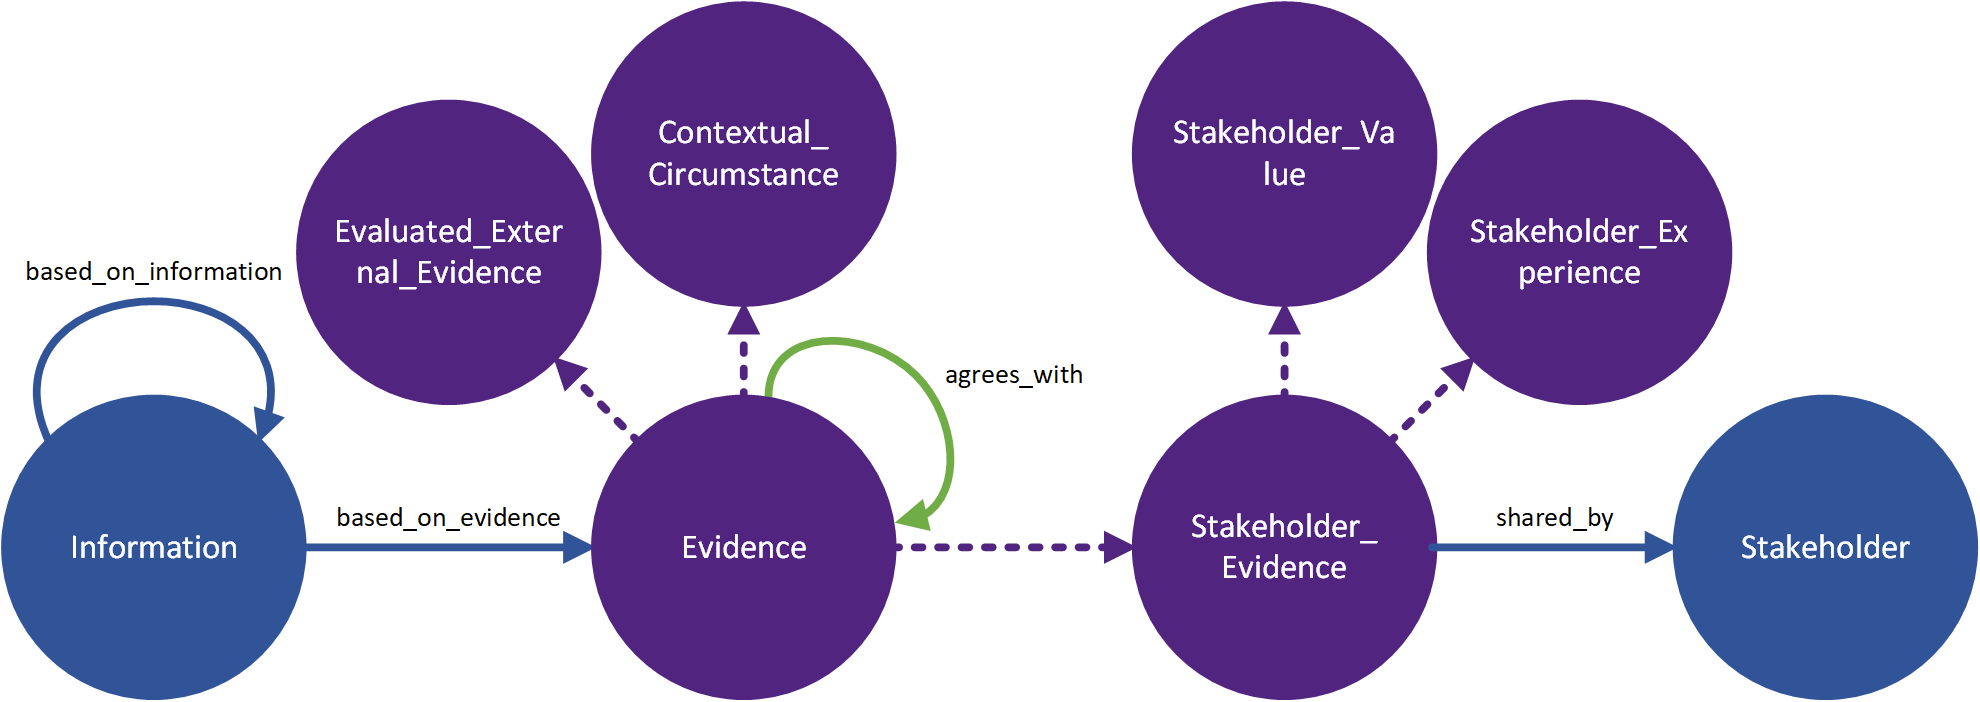
\includegraphics[width=14cm]{../../Images/04_Contribution/04_Consensus_Ontology.png}
  \caption{The consensus pattern that we have based on the reproducibility pattern. We have extended the reproducibility pattern with the object property $agrees\_with$. Code sample \ref{GODP_CON_LEV} extends the reproducibility pattern using GDOL.}
  \label{fig:consensus}
\end{figure}

\paragraph{Inferencing}
We can measure the consensus-level of an evidence source using the $agrees\_with$ object property. We extend the $based\_on\_evidence$ object property with a super property. When we base $In{\f}ormationX$ on $EvidenceA$, and $EvidenceA$ agrees with $EvidenceB$, the reasoner bases $In{\f}ormationX$ on $EvidenceB$ as well. Figure \ref{fig:consensus_inferred} presents the super property that infers this knowledge from the existing ontology structure.

\begin{figure}[H]
\centering
  
\includegraphics[width=17cm]{../../Images/Consensus_Inferred.png}
  \caption{The super property that infers the object property $based\_on\_evidence$ in Prot\'eg\'e.}
  \label{fig:consensus_inferred}
\end{figure}

The $agrees\_with$ object property is symmetric. If individual $A$ agrees with individual $B$, individual $B$ should also agree with individual $A$. Figure \ref{fig:consensus_transitive} presents the characteristics of the $agrees\_with$ object property.

\begin{figure}[H]
\centering
  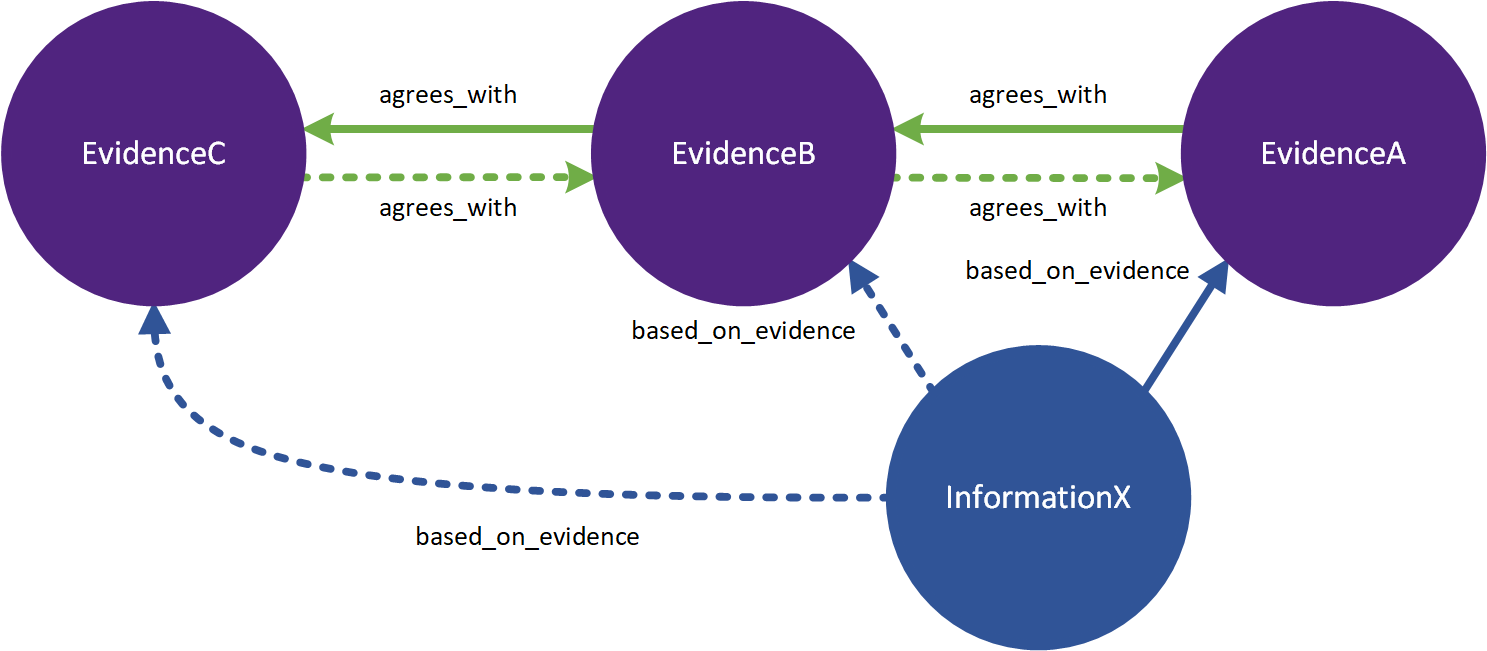
\includegraphics[width=13cm]{../../Images/04_Contribution/04_Consensus_Characteristics.png}
  \caption{An example of the impact of the symmetric characteristics of the $agrees\_with$ object property. The reasoner infers the dotted lines based on the super property figure \ref{fig:consensus_inferred} presents and the symmetric characteristics of $agrees\_with$.}
  \label{fig:consensus_transitive}
\end{figure}

\paragraph{Inconsistency}
The consensus pattern inherits the consistency validation from the reproducibility pattern. We describe the consistency of the reproducibility pattern in section \ref{rep_incons} \nameref{rep_incons}.

\paragraph{Generic ontology design pattern}
Code sample \ref{GODP_CON_LEV} presents the described solution into GDOL. We take the $Reproducibility\_Basic$ pattern, introduce the $agrees\_with$ object property, and extend the $based\_on\_evidence$ object property. 

\begin{lstlisting}[float,language=GDOL,caption={The GDOL code that extends the reproducibility pattern and results in the consensus pattern. We take the $Reproducibility\_Basic$ pattern, introduce the $agrees\_with$ object property, and extend the $based\_on\_evidence$ object property. Figure \ref{fig:consensus} presents the generic ontology design pattern.},label={GODP_CON_LEV}][H]
ontology Consensus = Reproducibility_Basic then
 ObjectProperty: agrees_with Domain: Evidence Range: Evidence Characteristics: Symmetric
 ObjectProperty: based_on_evidence SubPropertyChain: based_on_evidence o agrees_with SubPropertyOf: based_on_evidence
\end{lstlisting}

\paragraph{Constraints}
We define one consensus level for each individual classified as $Evidence$. We set the consensus-level to $1$. This consensus level ensures that each used evidence source has at least one other agreeable evidence source. The minimum consensus level can be adjusted depending on the environment. For example, in life-safety environments, the consensus level might be increased. We use the cardinality constraint $sh:minCount$ for the consensus detection: each individual classified as $Evidence$ should have at least one path $agrees\_with$.

\begin{lstlisting}[float,language=SHACL,caption={The SHACL shapes that detect when information does not meet the minimum consensus level.},label={SHACL_CON_LEV}][H]
UsedEvidenceShape a sh:NodeShape;
	sh:targetClass Evidence; 
	sh:property [
		sh:path agrees_with; 
		sh:severity sh:Violation; 
		sh:minCount 1; 
		sh:message "Consensus: ensure the evidence is in agreement with at least one additional evidence source."; ];
\end{lstlisting} 
\subsubsection{Conflict} \label{odp_conflict}
% Subsection structure:
% Problem: what is the generalized problem?
% 	Motivation: why is this problem scientifically important and/or interesting?
% Solution: conceptual description of solution, including formal definition of GODP and SHACL shapes.
% 	Illustration: images of GODP structure.
% 	(Statistical)Analysis: how does the solution solve the problem?
% 	Evaluation: are the results significant? What is the impact?
\paragraph{Detecting conflict}
Information that has conflicting evidence sources is less reliable compared to information that does not have conflicting evidence sources. For example, stakeholder experience that is conflicting with evaluated external evidence is less reliable compared to stakeholder experience that does not have any conflict. We define the number of evidence sources that causes a conflict with the decision-relevant information as the level of conflict. We define the level of conflict using the reproducibility of information. When information is reproducible by one evidence source, and this evidence source has one additional conflicting evidence source, the level of conflict is $1$. When the evidence source has two conflicting evidence sources, the level of conflict is $2$. Compared to a fuzzy approach that can classify certain conflict levels as, for example, $low$, $medium$, or $high$, the number-based approach makes it easier to compare conflict levels. We do not compare conflict-levels in this study.

\begin{center}
\large\color{document}{The conflict pattern validates information reliability by detecting conflicting evidence.} 
\end{center}

\paragraph{Ontology}
We define conflicting evidence as evidence that disagrees with another evidence source. The reproducibility pattern serves as a natural base for the conflict pattern. The reproducibility pattern provides the structure on which we create the conflict pattern using the object property $disagrees\_with$. Figure \ref{fig:conflict} presents the conflict pattern. We mark the extension of the conflict pattern in \textcolor{Red}{red}. We measure the level of conflict between evidence sources using the $disagrees\_with$ object property. For example, if two stakeholders have a different experience, the $disagrees\_with$ object property represents this conflicting stakeholder experience. 

\begin{figure}[H]
\centering
  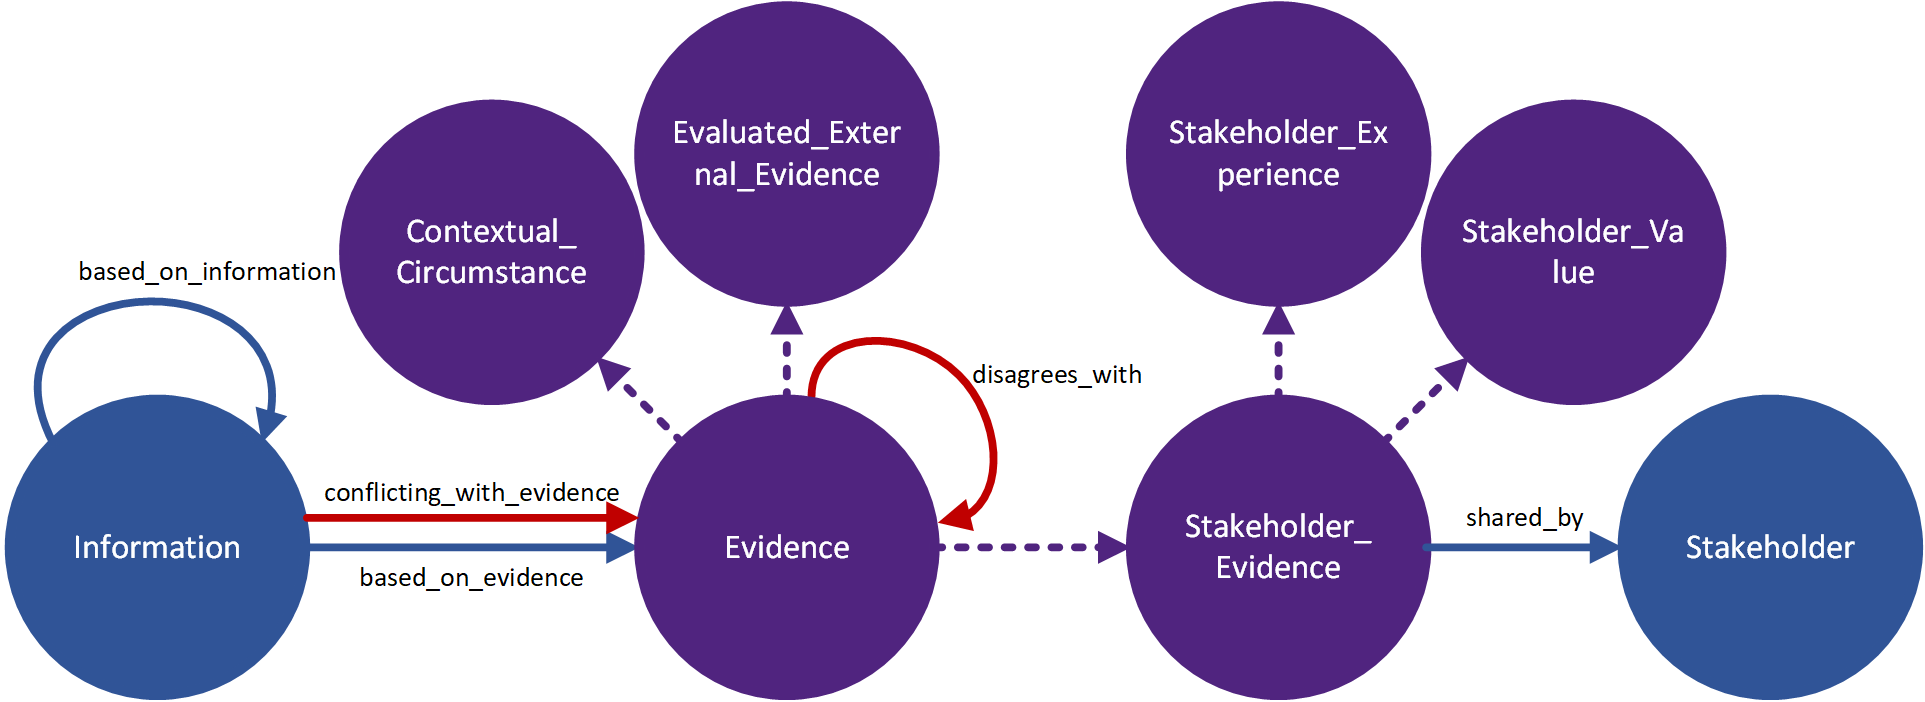
\includegraphics[width=14cm]{../../Images/04_Contribution/04_Conflict_Ontology.png}
  \caption{The conflict pattern uses the reproducibility pattern and extends it with the object property $disagrees\_with$. Code sample \ref{GODP_CONF_LEV} presents the GDOL code for instantiating the conflict pattern.}
  \label{fig:conflict}
\end{figure}

\paragraph{Inferencing}
We introduce an additional object property: $conflict\_with\_evidence$. When we base $In{\f}ormationX$ on $EvidenceA$, and $EvidenceA$ disagrees with $EvidenceB$, $In{\f}ormationX$ conflicts with $EvidenceB$. This conflict reduces trust in $In{\f}ormationX$. Figure \ref{fig:conflict_inferred} presents the super property that infers this knowledge from the existing ontology structure.

\begin{figure}[H]
\centering
  
\includegraphics[width=17cm]{../../Images/Conflict_Inferred.png}
  \caption{The configuration of the super property that infers the object property $conflict\_with\_evidence$ in Prot\'eg\'e.}
  \label{fig:conflict_inferred}
\end{figure}

$disagrees\_with$ is symmetric and irreflexive. Disagreement is always symmetric: if $StakeholderA$ disagrees with $StakeholderB$ on a specific subject, then $StakeholderB$ also disagrees with $StakeholderA$. Figure \ref{fig:conflict_irreflexive} presents the situation in which $disagrees\_with$ is symmetric and irreflexive.

\begin{figure}[H]
\centering
  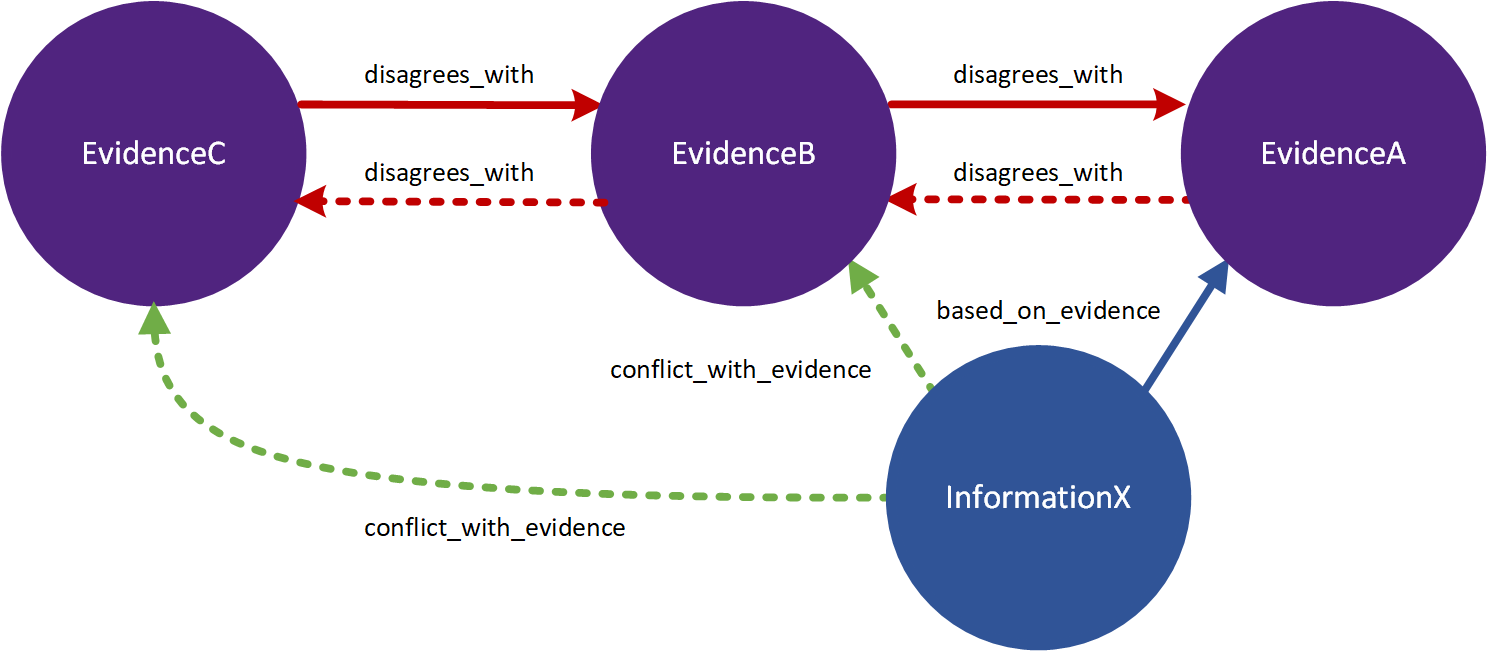
\includegraphics[width=13cm]{../../Images/04_Contribution/04_Conflict_Characteristics.png}
  \caption{The symmetric and irreflexive characteristics of $disagrees\_with$. The reasoner infers the dotted lines based on the super property figure \ref{fig:conflict_inferred} presents.}
  \label{fig:conflict_irreflexive}
\end{figure}

\paragraph{Inconsistency}
The consensus pattern inherits the consistency validation from the reproducibility pattern. We describe the consistency of the reproducibility pattern in section \ref{rep_incons} \nameref{rep_incons}.

Figure \ref{fig:conflict_transitive} presents the hypothetical situation in which $disagrees\_with$ is symmetric, transitive, and irreflexive. This situation results in an inconsistent ontology. The reasoner infers the $disagrees\_with$ object property on $EvidenceA$ based on the transitivity characteristic. This object property causes conflict with the irreflexive character of $disagrees\_with$. The transitivity helps us to discover disagreement chains and ensures we present the right conflict level to the decision-maker. Transitivity causes a problem: evidence cannot disagree with itself. When we combine the irreflexive and transitive characteristics, the reasoner might infer the $disagrees\_with$ object property on an evidence source. For example, we assume $R$ is transitive and irreflexive. By transitivity, we conclude $xRy \land yRx \rightarrow xRx$. However, this is not possible as $R$ should be irreflexive as well.

\begin{figure}[H]
\centering
  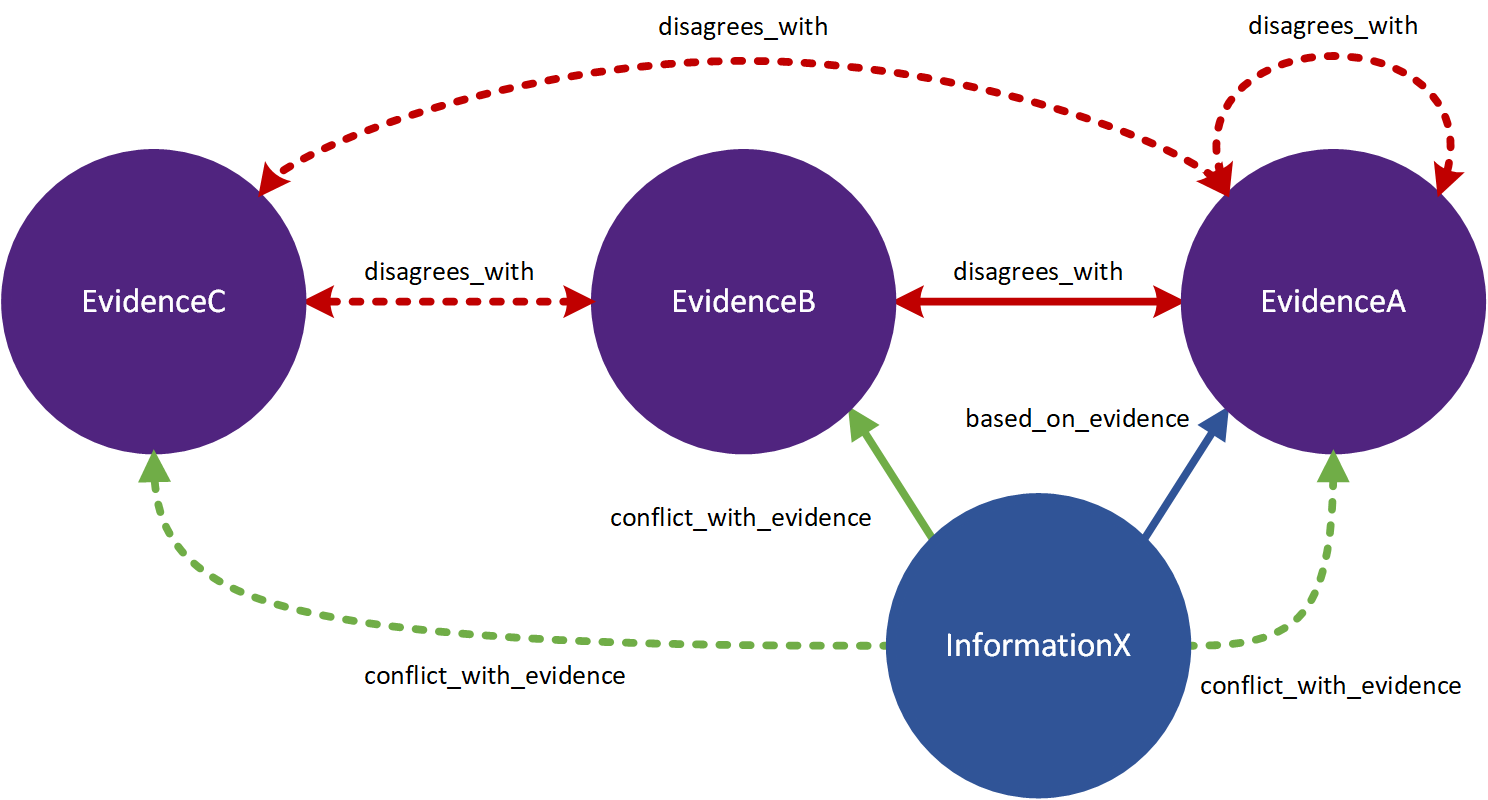
\includegraphics[width=13cm]{../../Images/Conflict_Transitive.png}
  \caption{The transitive characteristic of $disagrees\_with$ causes an inconsistent ontology. The reasoner infers the dotted lines based on the super property figure \ref{fig:conflict_inferred} presents.}
  \label{fig:conflict_transitive}
\end{figure}

\paragraph{Generic ontology design pattern}
Code sample \ref{GODP_CONF_LEV} presents the described solution into GDOL. We take the $Reproducibility\_Basic$ pattern and add the $disagrees\_with$ and $conflict\_with\_evidence$ object properties.

\begin{lstlisting}[float,language=GDOL,caption={The GDOL code that extends the reproducibility pattern and results in the conflict pattern. We take the $Reproducibility\_Basic$ pattern and add the $disagrees\_with$ and $conflict\_with\_evidence$ object properties.},label={GODP_CONF_LEV}][H]
ontology Conflict = Reproducibility_Basic then
  ObjectProperty: disagrees_with Domain: Evidence Range: Evidence Characteristics: Symmetric, Irreflexive
  ObjectProperty: conflict_with_evidence SubPropertyChain: based_on_evidence o disagrees_with SubPropertyOf: conflict_with_evidence
end
\end{lstlisting}

\paragraph{Constraints}
The conflict pattern requires the definition of a conflict level. Conflict reduces the reliability of the information and evidence. Therefore, we do not accept any conflict for our evidence and define the maximum conflict-level as $0$. Any conflict that the constraints detect immediately causes a violation. We use the cardinality constraint $sh:minCount$ for this detection: each individual classified as $In{\f}ormation$ should not have any path (object property) $conflict\_with\_evidence$.

\begin{lstlisting}[float,language=SHACL,caption={The SHACL shapes that detect if there is conflict. },label={SHACL_CONF_LEV}][H]
Used_InformationShape a sh:NodeShape;
	sh:targetClass Used_Information; 
	sh:property [
		sh:path conflict_with_evidence; 
		sh:severity sh:Violation; 
		sh:maxCount 0; 
		sh:message "Conflict detected. Please resolve the conflict or re-consider using this information."; ];
\end{lstlisting} 

\subsubsection{Pattern consolidation}
The decision ontology pattern reduces the complexity of the instantiation of the completeness, reproducibility, consensus, and conflict patterns.

\paragraph{Pattern dependencies}
We cannot reproduce information that does not exist. We validate the reproducibility of existing, and therefore, complete information. The consensus and conflict patterns have a similar dependency on the reproducibility pattern. When information is evidence-based, we can validate if the evidence agrees with other evidence (and define the level of consensus) or if information disagrees with other evidence (and define the level of conflict). 

\begin{center}
\large\color{document}{There is no consensus or conflict without reproducibility. There is no reproducibility without completeness.} 
\end{center}

\paragraph{Completeness and reproducibility using N-ary relations}
The completeness pattern validates the completeness of data properties and object properties. The reproducibility pattern validates the reproducibility of individuals using the object properties $based\_on\_evidence$ and $based\_on\_in{\f}ormation$. We need to relate a data property, containing decision-relevant information, to an object property. Figure \ref{fig:DecisionDesignPattern_NARY1} presents an example: $dataproperty1$ would be reproducible based on $based\_on\_evidence$. However, $dataproperty2$ would not be reproducible.

\begin{figure}[H]
\centering
  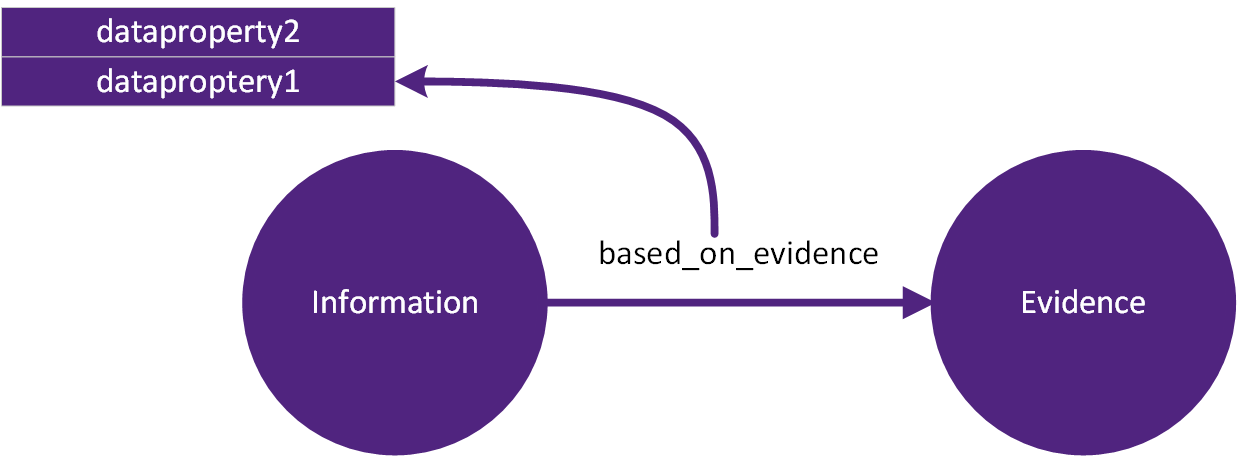
\includegraphics[width=10cm]{../../Images/04_Contribution/04_DecisionDesignPattern_NARY1.png}
  \caption{How can we reproduce $dataproperty1$ based on the object property $based\_on\_evidence$? However, $dataproperty2$ is not reproducible.}
  \label{fig:DecisionDesignPattern_NARY1}
\end{figure}

A property is a binary relation that relates two individuals \parencite{WEB16}. This concept makes it challenging to describe a relationship. In our case, we would describe the $based\_on\_evidence$ relationship with the data properties this relationship represents. We can describe object properties using annotations. Figure \ref{fig:DecisionDesignPattern_NARY2} presents the implementation of the annotation on the object property $based\_on\_evidence$ in Prot\'eg\'e, indicating that it $reproduces$ the $requirement\_cost$. 

\begin{figure}[H]
\centering
  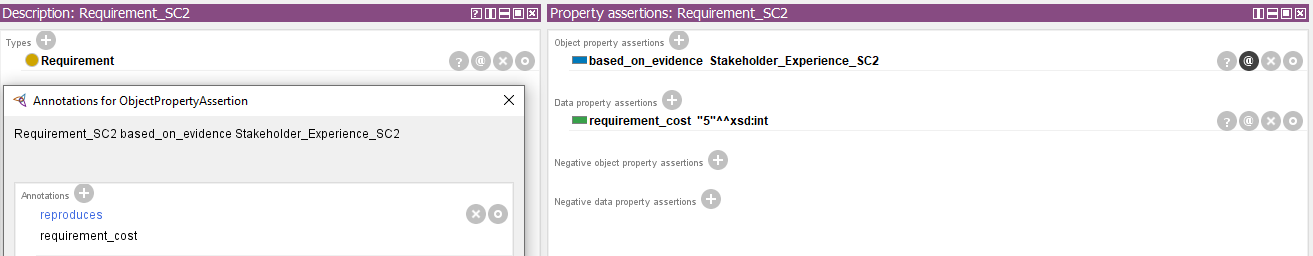
\includegraphics[width=16cm]{../../Images/04_Contribution/04_DecisionDesignPattern_NARY2.png}
  \caption{The implementation of the annotation on the object property $based\_on\_evidence$ in Prot\'eg\'e, indicating that it $reproduces$ the $requirement\_cost$.}
  \label{fig:DecisionDesignPattern_NARY2}
\end{figure}

However, annotation properties are merely descriptive and cannot define a characteristic of an object or data property \parencite{WEB12}. Therefore, the annotation properties are not suitable for inferencing or constraint validation. Additionally, we cannot use annotation properties to validate the reproducibility.

We define n-ary relations to solve this challenge \parencite{WEB16}. An n-ary relation introduces a new class for information that we would typically store in a data property. The new class hosts the actual information as data properties. We define three types of individuals for our purpose: $root$, $in{\f}ormation$, and $target$. The $root$ provides the context for the $in{\f}ormation$. The $in{\f}ormation$ stores the actual information in two data properties ($data\_value$ and $data\_description$), and the $target$ serves as the target for reproduction. We use the $data\_value$ to give an integer to the information. The $data\_description$ describes the value. We suggest setting the $data\_value$ to $0$ when the context does not require the use of the $data\_value$. Figure \ref{fig:root_information_target} presents the definitions.

\begin{figure}[H]
\centering
  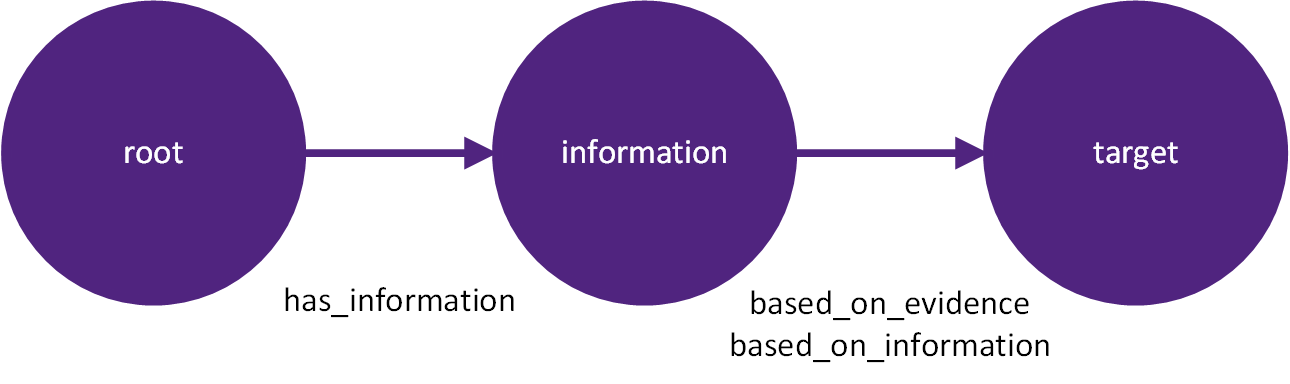
\includegraphics[width=10cm]{../../Images/04_Contribution/04_root_information_target.png}
  \caption{The $root$, $in{\f}ormation$, and $target$ individuals in n-ary relation.}
  \label{fig:root_information_target}
\end{figure}

Figure \ref{fig:DecisionDesignPattern_NARY3} presents an example of this concept. Class $r$, the root class, has two decision-relevant information properties: $n1$ and $n2$. These decision-relevant information properties have at least the $data\_value$ and $data\_description$ data properties. We classify them as $In{\f}ormation$. $n1$ and $n2$ are reproducible using the object properties $based\_on\_evidence$ or $based\_on\_in{\f}ormation$. We need to ensure that the completeness and reproducibility patterns function in this environment.

\begin{figure}[H]
\centering
  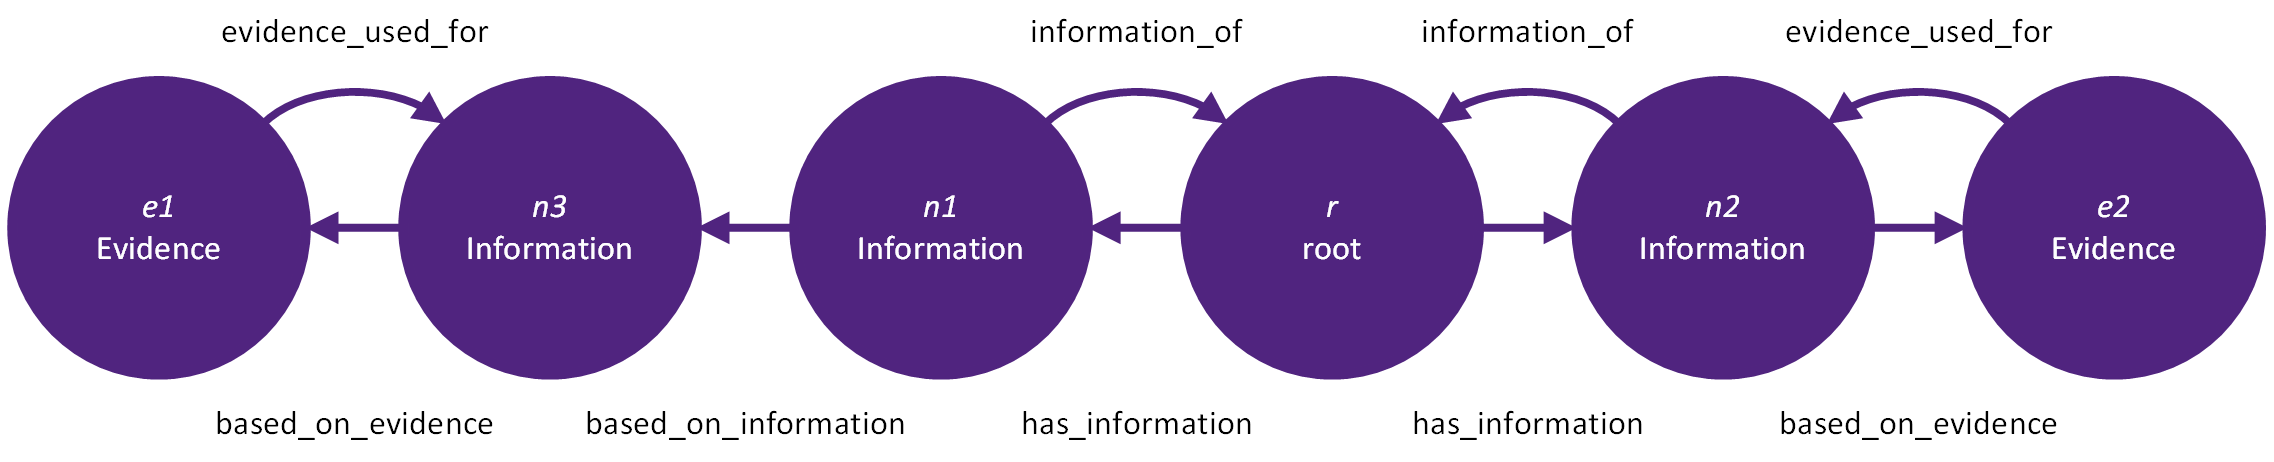
\includegraphics[width=17cm]{../../Images/04_Contribution/04_DecisionDesignPattern_NARY3.png}
  \caption{Class $r$ with two decision-relevant information properties: $n1$ and $n2$. These decision-relevant information properties have a $data\_value$ and a $data\_description$. $n1$ and $n2$ are reproducible using the object property $based\_on\_evidence$.}
  \label{fig:DecisionDesignPattern_NARY3}
\end{figure}

We validate the completeness of information using the $has\_information$ object property, including its range. We validate the reproducibility of information using the $based\_on\_evidence$ and $based\_on\_in{\f}ormation$ object properties.

\paragraph{\emph{Used} classes}
We use $Used\_*$ classes throughout the patterns to define the scope of the constraints. Each $Used\_*$ class is a subclass of its parent. We define the $Used\_*$ class in a way the reasoner classifies individuals that are relevant for the constraints. Figure \ref{fig:04_Used_Information} presents, for example, the $Used\_In{\f}ormation$ class. There might be a lot of individuals classified as $In{\f}ormation$. However, these individuals are only relevant to the decision-maker if the decision-maker uses them. The reasoner classifies individuals as $Used\_In{\f}ormation$ when they have the $in{\f}ormation\_of$ object property. We use the inverse of the $has\_in{\f}ormation\_*$ object property to infer that information is used in the context of a decision-relevant root individual. We use the $evidence\_used\_for$ object property to infer $Used\_Evidence$ similarly.  

\begin{figure}[H]
\centering
  
\includegraphics[width=12cm]{../../Images/04_Contribution/04_Used_Information.png}
  \caption{The $Used\_In{\f}ormation$ configuration in Prot\'eg\'e. The reasoner classifies individuals as $Used\_In{\f}ormation$ when they have the $in{\f}ormation\_of$ object property.}
  \label{fig:04_Used_Information}
\end{figure} 

\paragraph{Inferencing}
We use inferencing in the decision design pattern to infer the information types from the object property $has\_information\_*$. The completeness pattern uses the information generated by the reasoner to validate the existence of specific data properties. Figure \ref{fig:04_DDP_Inference} presents an example in which individual $A$ is connected to individual $B$ by $has\_information\_temperature$. We set the range of $has\_information\_temperature$ to the class $Temperature$. As a result, the reasoner infers that $B$ must be of type $Temperature$. This mechanism allows the completeness pattern to validate if individuals classified as $Temperature$ have specific data or object properties.

\begin{figure}[H]
\centering
  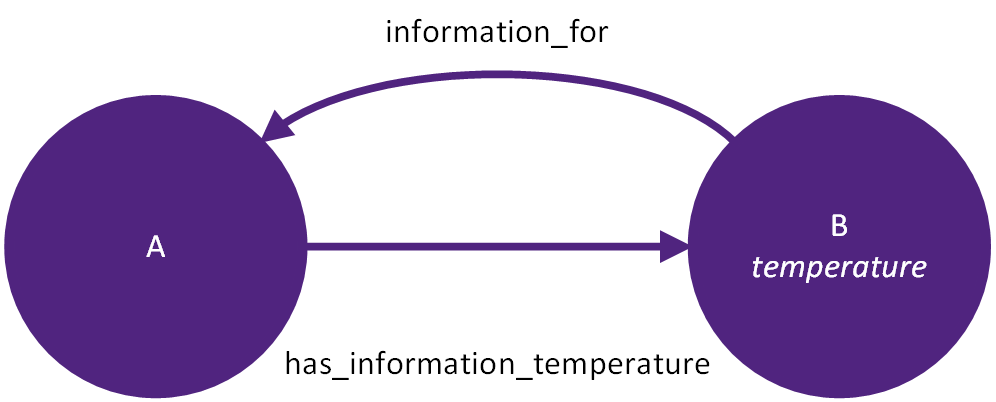
\includegraphics[width=8cm]{../../Images/04_Contribution/04_DDP_Inference.png}
  \caption{An example in which individual $A$ is connected to individual $B$ by $has\_information\_temperature$. We set the range of $has\_in{\f}ormation\_temperature$ to the class $Temperature$. As a result, the reasoner infers that $B$ must be of type $Temperature$.}
  \label{fig:04_DDP_Inference}
\end{figure}

\paragraph{Inconsistency}
We guard the consistency of the ontology using $DisjointClasses$. The $agrees\_with$ and $disagrees\_with$ object properties of the consensus and conflict patterns are naturally disjoint: when evidence $A$ agrees with evidence $B$, they cannot disagree at the same time. The decision design pattern inherits other inconsistency prevention mechanics from the completeness, reproducibility, consensus, and conflict patterns.

\paragraph{Generic ontology design pattern} \label{dop-godp}
The decision ontology pattern instantiates the completeness, reproducibility, consensus, and conflict patterns. These patterns have an overlap in their instantiation; for example, the consensus and conflict pattern both instantiate the $Reproducibility\_Base$. We reduce the overlap by defining new instantiation code. Code sample \ref{GODP_DDP_Instantiation_Basic} presents the instantiation code for the base ontology structure. The base instantiation code addresses the reproducibility, consensus, conflict, and a part of the completeness pattern. The base instantiation does not use any parameters.

\begin{lstlisting}[float,language=GDOL,caption={The base GDOL instantiation code for the decision ontology pattern. The instantiation code is a combination of the completeness, reproducibility, consensus, and conflict patterns.},label={GODP_DDP_Instantiation_Basic}][H]
pattern DecisionOntologyPattern_Basic = Reproducibility_Basic then
 %% Consensus pattern without reproducibility pattern
 ObjectProperty: agrees_with Domain: Evidence Range: Evidence Characteristics: Transitive, Symmetric
 ObjectProperty: based_on_evidence SuperPropertyOf: based_on_evidence o agrees_with SubPropertyOf: based_on_evidence
 %% Conflict pattern without reproducibility pattern
 ObjectProperty: disagrees_with Domain: Evidence Range: Evidence Characteristics: Symmetric, Irreflexive
 ObjectProperty: conflict_with_evidence SuperPropertyOf: based_on_evidence o disagrees_with SubPropertyOf: conflict_with_evidence
 %% Completeness pattern
 Completeness_dp [data_value][Information][xsd:int] %% Data property and information class as parameters
 Completeness_dp [data_description][Information][xsd:string] %% Data property and information class as parameters
 %% Used information
 Object Property: information_of InverseOf: has_information
 Class: Used_Information EquivalentTo: information_of some owl:Thing
 %% Used evidence
 Object Property: evidence_used_for InverseOf: based_on_evidence
 Class: Used_Evidence EquivalentTo: evidence_used_for some Information 
\end{lstlisting}
 
Figure \ref{fig:DecisionDesignPattern} presents the instantiated decision ontology pattern. This ontology does not include context. We took the \textcolor{Violet}{violet} edges and nodes from the evidence-based management pattern, the \textcolor{DarkBlue}{blue} edges and nodes from the reproducibility pattern, the \textcolor{Red}{red} edges from the conflict pattern, and the \textcolor{Green}{green} edge from the consensus pattern. The completeness pattern does not include structural elements.
 
\begin{figure}[H]
\centering
  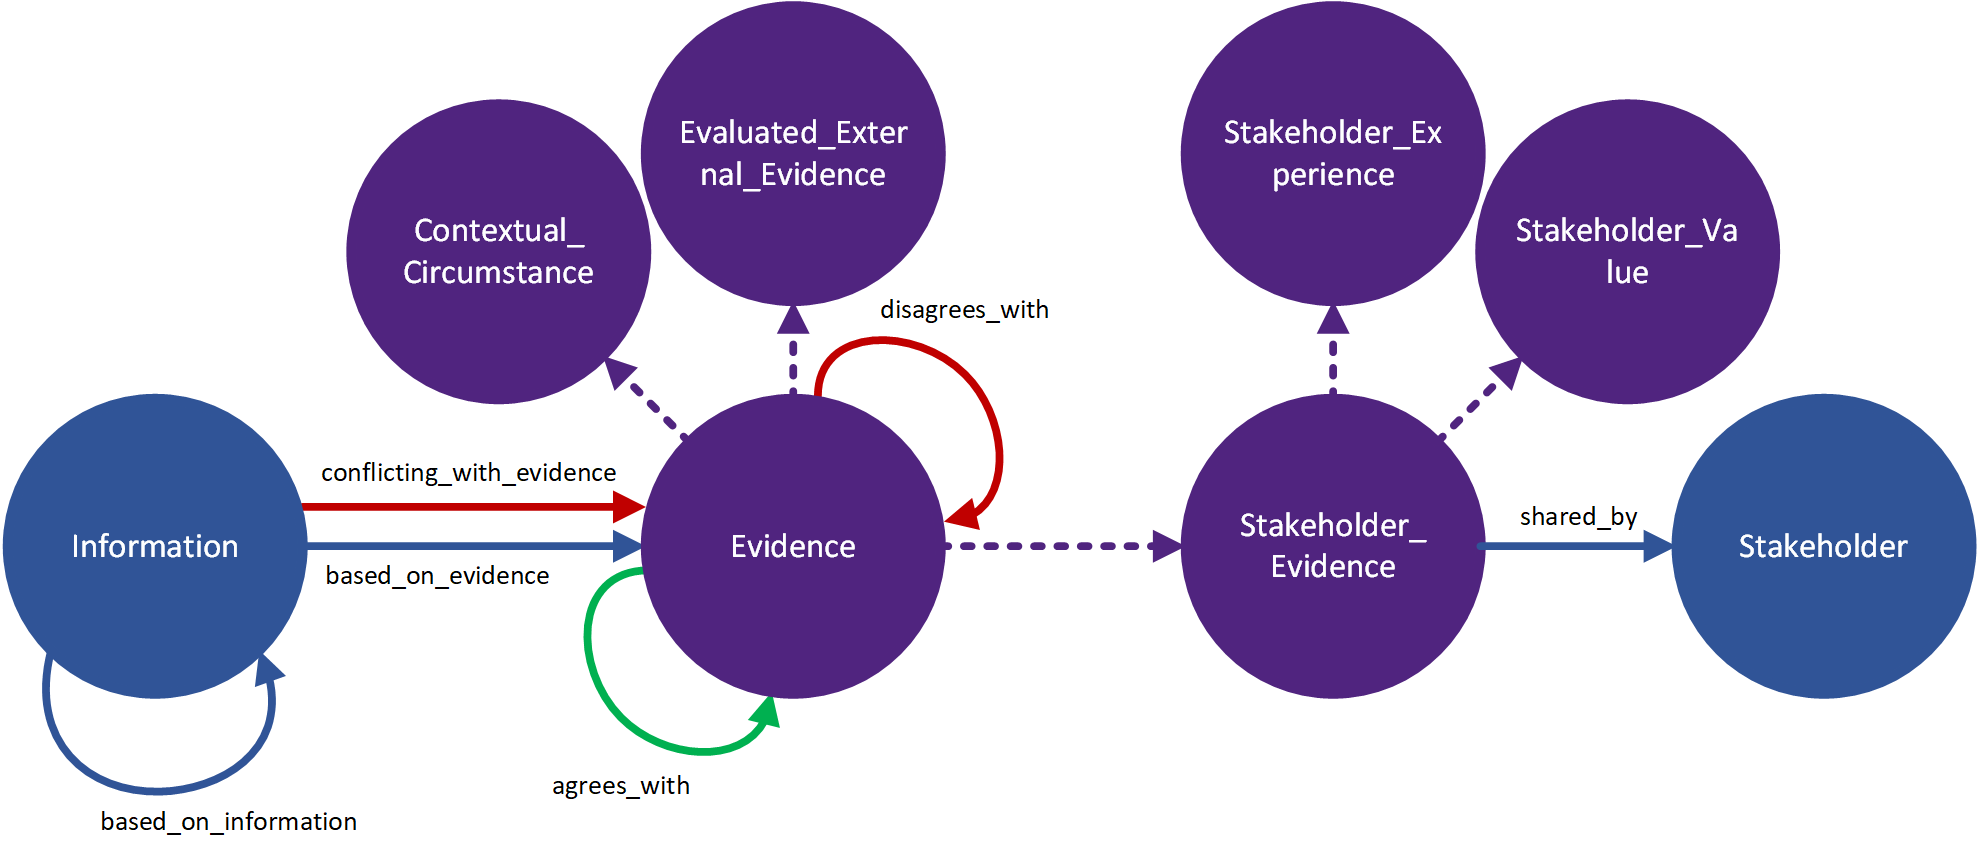
\includegraphics[width=15cm]{../../Images/04_Contribution/04_DecisionDesignPattern.png}
  \caption{The instantiated decision ontology pattern without context. We took the \textcolor{Violet}{violet} edges and nodes from the evidence-based management pattern, the \textcolor{DarkBlue}{blue} edges and nodes from the reproducibility pattern, the \textcolor{Red}{red} edges from the conflict pattern, and the \textcolor{Green}{green} edge from the consensus pattern.}
  \label{fig:DecisionDesignPattern}
\end{figure}

The completeness and reproducibility patterns require a context-specific instantiation. We instantiate a new context-specific ontology structure for every information type that decision-makers use to make a decision. We use parameter $i$ to represent this class. Code sample \ref{GODP_DDP_Instantiation_Context} presents the context-specific instantiation code. 

\begin{lstlisting}[float,language=GDOL,caption={The context-specific GDOL instantiation code to instantiate the decision design pattern. The code is a combination of the context-specific instantiation code of the completeness and reproducibility patterns.},label={GODP_DDP_Instantiation_Context}][H]
pattern DecisionOntologyPattern_Context [Class: i; Class: r] = 
 Completeness_op[has_information[i]; r; i] %% Object property, root class, and information class as parameters
\end{lstlisting}

\paragraph{Constraints}
We need to combine the basic and context-dependent constraints of the completeness, reproducibility, consensus, and conflict patterns. The constraints of the reproducibility and conflict patterns target the $Used\_In{\f}ormation$ class. Code sample \ref{SHACL_DDP_Basic} combines the constraints for these two patterns into one SHACL shape. 

\begin{lstlisting}[float,language=SHACL,caption={This code sample combines the constraints of the reproducibility, consensus, and conflict patterns. We have merged parts of the reproducibility and consensus patterns.},label={SHACL_DDP_Basic}][H]
UsedInformationShape a sh:NodeShape;
	sh:targetClass Used_Information; 
	sh:property [
		sh:or (
			[sh:path based_on_information; sh:minCount 1;]
			[sh:path based_on_evidence; sh:minCount 1;]
		)
		sh:severity sh:Violation; 
		sh:minCount 1; 
		sh:message "Reproducibility: increase the number of evidence sources for this information."; ];
	sh:targetClass Information; 
	# Conflict pattern
	sh:property [
		sh:path conflict_with_evidence; 
		sh:severity sh:Violation; 
		sh:maxCount 0; 
		sh:message "Conflict detected. Please resolve the conflict or re-consider using this information."; ];
\end{lstlisting}

Code sample \ref{SHACL_REP_SH} is part of the reproducibility pattern and presents the constraints that validate if $Stakeholder\_Evidence$ is $shared\_by$ a stakeholder. Code sample \ref{SHACL_CON_LEV} presents the constraints that validate the consensus pattern. We include both code samples as-is into the decision ontology pattern.

We instantiate the contextual constraints multiple times per scenario, depending on the need of the scenario. The completeness pattern is context-sensitive. Code sample \ref{SHACL_COM_DP} presents the only context-sensitive constraints we use in the decision design pattern.